\documentclass[12pt]{beamer}
%\documentclass[20pt,handout]{beamer}
\usetheme{Darmstadt}
\usepackage{graphicx}
%\usepackage[german]{babel}
\usepackage{ngerman}
\usepackage[T1]{fontenc}
\usepackage[utf8]{inputenc}
\usepackage{tikz}
\setbeamertemplate{footline}[frame number]

\newcommand{\cc}[1]{\includegraphics[height=4mm]{img/#1.png}\hspace{1mm}}
\usepackage{ifthen}
\newcommand{\license}[2][]{\\#2\ifthenelse{\equal{#1}{}}{}{\\\scriptsize\url{#1}}}
\usepackage{textcomp}
\usepackage{hyperref}

\pgfdeclareimage[height=.6cm]{c3d2logo}{./img/c3d2.pdf}

\pgfdeclarelayer{foreground}
\pgfsetlayers{main,foreground}
\logo{\pgfputat{\pgfxy(-1,0)}{\pgfbox[center,base]{\pgfuseimage{c3d2logo}}}}

\title{Digitale Selbstverteidigung}
\author{\small Marius Melzer (marius@rasumi.net) \\\large Chaos Computer Club Dresden}
\date{28.01.2016}

\begin{document}
\maketitle

\section{Einleitung}
\subsection{}

\begin{frame}
    \frametitle{Chaos Computer Club}
    \begin{center}
	\includegraphics[height=0.2\textheight]{img/chaosknoten.png}
    \end{center}	
    \begin{itemize}
      \item<1-> Verein wurde 1981 gegr"undet (\url{https://ccc.de})
      \item<2-> Aktuell > 6000 Mitglieder
      \item<3-> Technologie zum gesellschaftlichen Nutzen (und nicht ihrem Schaden)
      \item<3-> Betreibt u.a. "Offentlichkeitsarbeit und Politikberatung
    \end{itemize}
\end{frame}

\begin{frame}
  \frametitle{Chaos Computer Club}
  \begin{figure}
    \includegraphics[height=0.7\textheight]{img/fingerabdruck.jpg}
  \end{figure}
\end{frame}

\begin{frame}
  \frametitle{Chaos Computer Club}
  \begin{figure}
    \includegraphics[height=0.7\textheight]{img/trojaner.png}
  \end{figure}
\end{frame}

\begin{frame}
    \frametitle{Chaos Computer Club}
    \begin{center}
	\includegraphics[height=0.1\textheight]{img/c3d2_logo.png}
    \end{center}
    \begin{itemize}
      \item<1-> Chaos Computer Club Dresden (\url{https://c3d2.de})
      \item<2-> Datenspuren: Herbst 2016 (\url{https://datenspuren.de})
      \item<3-> Podcasts (\url{https://c3d2.de/radio.html})
      \item<4-> Chaos macht Schule (\url{https://c3d2.de/schule.html})
    \end{itemize}
\end{frame}

\begin{frame}
    \frametitle{Bundespräsident Gauck zur NSA-Überwachung}
    \begin{center}
      ``Wir wissen z.B., dass es nicht so ist, wie bei der Stasi und dem KGB, dass es dicke Aktenbände gibt, wo unsere Gesprächsinhalte alle aufgeschrieben und schön abgeheftet sind. Das ist es nicht.''
      (Gauck, 30.06.2013 im ZDF-Sommerinterview)
    \end{center}
\end{frame}

\begin{frame}
    \frametitle{Stasi vs. NSA}
    \begin{center}
      \includegraphics[height=0.7\textheight]{img/akten1.png}
    \end{center}
\end{frame}

\begin{frame}
    \frametitle{Stasi vs. NSA}
    \begin{center}
      \includegraphics[height=0.7\textheight]{img/akten2.png}
    \end{center}
\end{frame}

\section{Einführung}
\subsection{}

\begin{frame}
  \frametitle{Wer sind potenzielle Angreifer?}
  \begin{itemize}
    \item<1-> andere Nutzer (eines Dienstes)
    \item<2-> Fremde (``Hacker'')
    \item<3-> Dienstanbieter (z.B. für Werbung)
    \item<4-> staatliche Institutionen, Netzbetreiber
  \end{itemize}
\end{frame}

\begin{frame}
    \frametitle{Wie kommunizieren wir im Internet?}
    \begin{center}
      \includegraphics[height=5cm]{img/c-s.png}
    \end{center}
\end{frame}

\begin{frame}
    \frametitle{Server im Rechenzentrum}
    \begin{center}
      \includegraphics[height=5cm]{img/data_center.jpg}
    \end{center}
\end{frame}

\begin{frame}
    \frametitle{Internetknoten (Router)}
    \begin{center}
      \includegraphics[height=5cm]{img/internet_cable_map.png}
    \end{center}
\end{frame}

\begin{frame}
    \frametitle{Internetknoten (DE-CIX in Frankfurt)}
    \begin{center}
      \includegraphics[height=5cm]{img/de_cix.png}
    \end{center}
\end{frame}

\begin{frame}
    \frametitle{Föderation}
    \begin{center}
      \includegraphics[height=5cm]{img/fed.png}
    \end{center}
\end{frame}

\begin{frame}
    \frametitle{P2P}
    \begin{center}
      \includegraphics[width=7cm]{img/direkt.png}
    \end{center}
\end{frame}

\begin{frame}
    \frametitle{Was ist zu schützen?}
    \begin{center}
      \includegraphics[height=5cm]{img/fed.png}
    \end{center}
\end{frame}

\section{Geräte}
\subsection{}

\begin{frame}
  \frametitle{Problematisches Verhalten von Software}
  \begin{itemize}
    \item<1-> Sicherheitslücken
    \item<2-> Backdoors
    \item<3-> Unerwünschte Funktionalität
  \end{itemize}
\end{frame}

\begin{frame}
  \frametitle{Backdoors}
  \begin{center}
    \includegraphics[width=10cm]{img/backdoor-windows}
  \par\end{center}
\end{frame}

\begin{frame}
  \frametitle{Backdoors}
  \begin{center}
    \includegraphics[width=10cm]{img/backdoor-av}
  \par\end{center}
\end{frame}

\begin{frame}
    \frametitle{Unerwünschte Funktionalität}
    \begin{center}
      \includegraphics[width=0.7\textwidth]{img/windows10.png}
    \end{center}
\end{frame}

\begin{frame}
  \frametitle{Unerwünschte Funktionalität}
  \begin{center}
    \includegraphics[width=7cm]{img/backdoor-apps}
  \par\end{center}
\end{frame}

\begin{frame}
  \frametitle{Unerwünschte Funktionalität}
  \begin{center}
    \includegraphics[width=10cm]{img/backdoor-android}
  \par\end{center}
\end{frame}

\begin{frame}
    \frametitle{Wie schütze ich meine Geräte?}
    \begin{itemize}
      \item (Virenscanner)
      \item Firewall
      \item Aktuelle und vertrauenswürdige Software
    \end{itemize}
\end{frame}

\begin{frame}
    \frametitle{Vertrauenswürdige Software?}
    \begin{center}\Large
        Einer Software, die nicht quelloffen ist, kann man nicht vertrauen
    \end{center}
\end{frame}

\begin{frame}
  \frametitle{Kompilierung von Software}
  \begin{center}
    \includegraphics[width=10cm]{img/compilation-process}
  \par\end{center}
\end{frame}

\begin{frame}
  \frametitle{Probleme von proprietärer Software}
  \begin{itemize}
    \item<2-> Kontrolle unterliegt einer Organisation
    \item<3-> Transparenz und Sicherheit
  \end{itemize}
\end{frame}

\begin{frame}
  \frametitle{Strategien moderner IT-Unternehmen}
  \begin{itemize}
    \item<2-> Hardware
    \item<3-> Software
    \item<4-> Internetdienste
    \item<5-> ... aus einer Hand
  \end{itemize}
\end{frame}

\begin{frame}
  \frametitle{Strategien moderner IT-Unternehmen}
  \begin{itemize}
    \item<2-> Fehlende Interoperabilität
    \item<3-> vorgegebene Dienste und Programme
    \item<4-> keine ausreichenden Nutzerrechte
    \item<5-> Kopierschutz, Online-Zwang, ...
  \end{itemize}
\end{frame}

\begin{frame}
  \frametitle{Strategien moderner IT-Unternehmen}
  \begin{center}
    ``Tie all of our products together, so we further lock customers into our ecosystem'' (Steve Jobs)
  \end{center}
\end{frame}

\begin{frame}{Das GNU Projekt}
  \begin{columns}
    \column{6cm}

    \begin{itemize}
      \item Begonnen von Richard Stallman im Jahr 1984 
      \item Gründung der Free Software Foundation im Jahr 1985 
    \end{itemize}

    \column{7cm}

    \begin{center}
      \includegraphics[width=4.5cm]{img/stallman}
    \par\end{center}

    \begin{center}
      \includegraphics[width=5cm]{img/logo-fsf}
    \par\end{center}
  \end{columns}
\end{frame}

\begin{frame}{Firefox und Thunderbird}
  \begin{columns}
    \column{6cm}

    \textbf{Firefox}
    \begin{itemize}
      \item Browser
    \end{itemize}

    \vspace{0.5cm}

    \textbf{Thunderbird}
    \begin{itemize}
      \item Email-Programm
    \end{itemize}

    \column{5cm}

    \begin{center}
      \includegraphics[width=2cm]{img/firefox.png}
    \par\end{center}
    \begin{center}
      \includegraphics[width=2cm]{img/thunderbird.png}
    \par\end{center}
  \end{columns}
\end{frame}

\begin{frame}{LibreOffice}
  \begin{columns}
    \column{6cm}

    \begin{itemize}
      \item Textverarbeitung
      \item Tabellenkalkulation
      \item Präsentationen
      \item Formeleditor
      \item nutzt Open Document Format zur Speicherung
    \end{itemize}

    \column{5cm}

    \begin{center}
      \includegraphics[width=5cm]{img/LibreOffice}
    \par\end{center}
  \end{columns}
\end{frame}

\begin{frame}{Freie Software für Android}
  \begin{columns}
    \column{6cm}

    \textbf{F-Droid}
    \begin{itemize}
      \item Installationsdienst für freie Android-Software
    \end{itemize}

    \vspace{0.5cm}

    \textbf{Signal}
    \begin{itemize}
      \item Verschlüsselter Nachrichtenaustausch
      \item Verschlüsselte Speicherung
    \end{itemize}

    \column{5cm}

    \begin{center}
      \includegraphics[width=2cm]{img/F-Droid_Logo_2}
    \par\end{center}
    \begin{center}
      \includegraphics[width=2cm]{img/TextSecure_Icon}
    \par\end{center}
  \end{columns}
\end{frame}

\begin{frame}{Replicant}
  \begin{columns}
    \column{6cm}
    \begin{itemize}
      \item basiert auf Android
      \item Ziel, alle proprietären Komponenten durch freie zu ersetzen
      \item Einbindung von F-Droid
      \item \textbf{Problem:} Verlust der Garantie bei Installation
    \end{itemize}
    \column{5cm}
    \begin{center}
      \includegraphics[width=2cm]{img/Replicant_logo_alpha}
    \par\end{center}
  \end{columns}
\end{frame}

\begin{frame}{Linux}
  \begin{columns}
    \column{8cm}
    \begin{itemize}
      \item Weit verbreitet als Server-Betriebssystem
      \item Bekannte Desktop-Varianten: 

      \begin{itemize}
        \item Ubuntu/Debian Linux
        \item Linux Mint
      \end{itemize}
      \item Können als Live-System ausprobiert werden
      \item Integrierte Software für Verschlüsselung, Webbrowsing, E-Mail, Textverarbeitung
      etc.
    \end{itemize}
    \column{6cm}

    \begin{center}
      \includegraphics[width=3cm]{img/Tux}
    \par\end{center}
  \end{columns}
\end{frame}

\begin{frame}
  \frametitle{Linux}
  \begin{center}
    \includegraphics[width=10cm]{img/gnome}
  \par\end{center}
\end{frame}

\begin{frame}
    \frametitle{Was ist zu schützen?}
    \begin{center}
      \includegraphics[height=5cm]{img/fed-clients.png}
    \end{center}
\end{frame}

\section{Inhalte}
\subsection{}

\begin{frame}
    \frametitle{Tempora}
    \includegraphics[height=0.7\textheight]{img/spiegel-tempora.png}
\end{frame}

\begin{frame}
    \frametitle{Verschlüsselung: symmetrisch}
    \begin{center}
	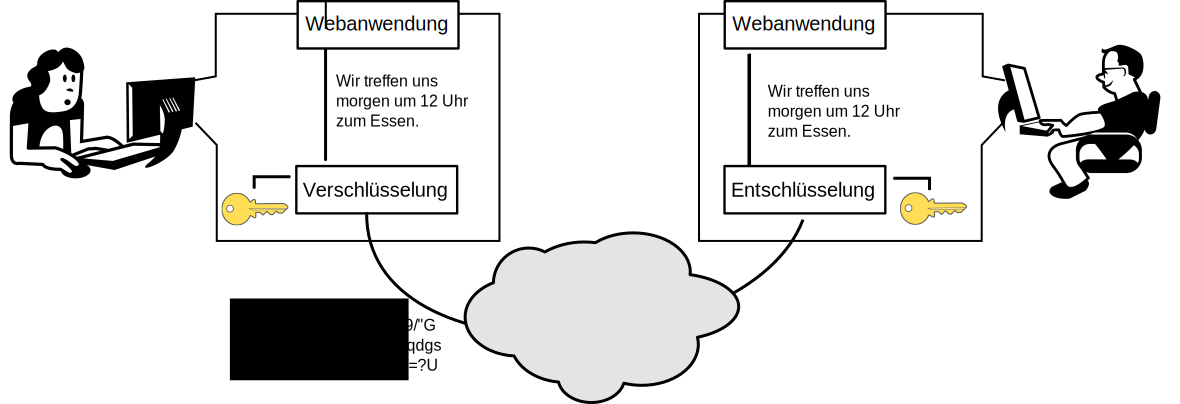
\includegraphics[width=\textwidth]{img/krypto.pdf}
    \end{center}	
\end{frame}

\begin{frame}
    \frametitle{Verschlüsselung: asymmetrisch}
    \includegraphics[height=0.7\textheight]<2->{img/asym_encryption.png}
\end{frame}

\begin{frame}
    \frametitle{Transportwegverschlüsselung}
      SSL = Secure Socket Layer / TLS = Transport Layer Security
    \vfill
    \begin{center}
      
\includegraphics[width=0.8\textwidth]{img/tls.pdf}
    \end{center}
\end{frame}

\begin{frame}
    \frametitle{SSL im Browser}
    \begin{center}
	\includegraphics[height=0.7\textheight]{img/ssl_special.png}
    \end{center}
\end{frame}

\begin{frame}
    \frametitle{Zertifizierungsstellen}
    \begin{center}
      \includegraphics[height=5cm]<2->{img/zertifikate.png}
    \end{center}
\end{frame}

\begin{frame}
  \frametitle{HTTPS Everywhere}
    \begin{center}
      \includegraphics[height=5cm]{img/https-everywhere.png}
    \end{center}
\end{frame}

\begin{frame}
    \frametitle{Was ist zu schützen?}
    \begin{center}
      \includegraphics[height=5cm]{img/fed-clients-comm.png}
    \end{center}
\end{frame}

\begin{frame}
    \frametitle{Prism}
    \includegraphics[height=0.7\textheight]{img/prism.jpg}
\end{frame}

\begin{frame}
  \frametitle{Dezentrale Dienste}
    \begin{columns}
        \begin{column}{5cm}
            \begin{center}
                
\includegraphics[height=0.2\textheight]{img/mail.pdf} \\
                E-Mail \\
                \vspace{1cm}
                \includegraphics[height=0.2\textheight]{img/jabber.png}
            \end{center}
        \end{column}
        \begin{column}{5cm}
            \begin{center}
                \includegraphics[height=0.2\textheight]{img/owncloud.png} \\
                \vspace{1cm}
                \includegraphics[width=0.8\textwidth]{img/sandstorm.png}
            \end{center}
        \end{column}
    \end{columns}
\end{frame}

\begin{frame}
  \frametitle{Ende-zu-Ende-Verschlüsselung}
  \begin{itemize}
    \item<1-> GPG für E-Mails
    \item<2-> OTR für Jabber:
      \begin{itemize}
        \item Pidgin mit OTR-Plugin für Linux und Windows
        \item ChatSecure oder Xabber für Android
        \item Adium für Mac, ChatSecure für iOS
      \end{itemize}
    \item<3-> palava.tv, talky.io, Tox, Linphone für Videotelefonie
    \item<4-> Signal
  \end{itemize}
\end{frame}

\begin{frame}
  \frametitle{E-Mail-Selbstverteidigung}
  \begin{center}
    \includegraphics[height=0.5\textheight]{img/emailselfdefense.png}
    \begin{itemize}
      \item https://emailselfdefense.fsf.org/de/
    \end{itemize}
  \end{center}
\end{frame}

\begin{frame}
  \frametitle{Signal}
    \begin{center}
      \includegraphics[height=6cm]{img/textsecure1.png}
      \hspace{0.5cm}
      \includegraphics[height=6cm]{img/textsecure2.png}
    \end{center}
\end{frame}

\begin{frame}
  \frametitle{Ich will etwas von einem anderen Nutzer}
    \begin{center}
      \includegraphics[height=5cm]{img/fed-end-to-end.png}
    \end{center}
\end{frame}

\section{Metadaten}
\subsection{}

\begin{frame}
    \frametitle{Metadaten im WWW}
    \begin{center} 
        \includegraphics<1>[width=0.7\textwidth]{img/lightbeam_1.png}
        \includegraphics<2>[width=0.7\textwidth]{img/lightbeam_2.png}
    \end{center}
\end{frame}

\begin{frame}
  \frametitle{Metadaten - VDS}
  \begin{itemize}
    \item Handynetz
      \begin{itemize}
        \item Telefonnummern
        \item Zeitpunkt und Dauer (Telefonate, SMS)
        \item Funkzelle (Ort)
      \end{itemize}
    \item Internet
      \begin{itemize}
        \item IP-Adresse (= ungefährer Ort)
        \item Alle Verbindungen
        \item Email: Adressen von Sender und Empfänger, Zugriff
      \end{itemize}
  \end{itemize}
\end{frame}

\begin{frame}
    \frametitle{Metadaten}
    \begin{center}
      \includegraphics[height=0.7\textheight]{img/wekillpeople.jpg}
    \end{center}
\end{frame}

\begin{frame}
    \frametitle{Metadaten - VDS}
    \includegraphics[height=0.7\textheight]{img/maltespitz.png}
\end{frame}

\begin{frame}
    \frametitle{Google Takeout}
    \begin{center}
      \includegraphics[width=0.8\textwidth]<1>{img/google_heat_1.png}
      \includegraphics[width=0.8\textwidth]<2>{img/google_heat_2.png}
    \end{center}
\end{frame}

\begin{frame}
    \frametitle{Zeitstempel}
    \begin{center}
      \only<1>{
        \includegraphics[width=0.9\textwidth]{img/punch_1.png}
        \\ \hfill \small Alan, Microblogging
      }

      \only<2>{
        \includegraphics[width=0.9\textwidth]{img/punch_2.png}
        \\ \hfill \small Bob, Microblogging
      }

      \only<3>{
        \includegraphics[width=0.9\textwidth]{img/punch_3.png}
        \\ \hfill \small Charlie, Github
      }
    \end{center}
\end{frame}

\begin{frame}
  \frametitle{Tor}
  \begin{center}
    \includegraphics[height=0.8\textheight]{img/torbrowser1.png}
  \end{center}
\end{frame}

\begin{frame}
    \frametitle{Tor}
    \includegraphics[height=0.7\textheight]{img/tor1.png}
    \\{\small \href{https://www.torproject.org/images/htw1.png}{Grafik}: \href{https://creativecommons.org/licenses/by/3.0/us/}{\cc{by}} The Tor Project}
\end{frame}

\begin{frame}
    \frametitle{Tor}
    \includegraphics[height=0.7\textheight]{img/tor2.png}
    \\{\small \href{https://www.torproject.org/images/htw2.png}{Grafik}: \href{https://creativecommons.org/licenses/by/3.0/us/}{\cc{by}} The Tor Project}
\end{frame}

\begin{frame}
    \frametitle{Tor}
    \includegraphics[height=0.7\textheight]{img/tor3.png}
    \\{\small \href{https://www.torproject.org/images/htw3.png}{Grafik}: \href{https://creativecommons.org/licenses/by/3.0/us/}{\cc{by}} The Tor Project}
\end{frame}

\begin{frame}
  \frametitle{Disconnect, Privacy Badger, Ghostery}
  \begin{center}
    \includegraphics[height=0.7\textheight]{img/disconnectme.jpg}
  \end{center}
\end{frame}

\section{Fazit}
\subsection{}

\begin{frame}
  \frametitle{Fazit}
  \begin{center}
    \begin{itemize}
      \item Verschlüsselung nutzen (Inhalte)
      \item Anonymisieren (Metadaten)
      \item Dezentrale Dienste nutzen (Inhalte + Metadaten)
      \item Endgeräte schützen
    \end{itemize}

    \vspace{5mm}
    \href{https://github.com/c3d2/cms-nsa}{Folien}: \href{https://creativecommons.org/licenses/by-sa/4.0/}{\cc{by-sa}} Chaos Computer Club Dresden \\
    \vspace{4mm}
    CMS Dresden: schule@c3d2.de
  \end{center}
\end{frame}

\end{document}
